\documentclass[a4paper, 11pt]{article}
\usepackage{fullpage} 
\usepackage[margin=1cm]{geometry}
\usepackage{graphicx}
\usepackage{enumitem}
\usepackage{fancyhdr}
\usepackage{multicol}
\usepackage{xhfill}
\usepackage{changepage}
\usepackage{listings}
\usepackage{color}

\definecolor{dkgreen}{rgb}{0,0.6,0}
\definecolor{gray}{rgb}{0.5,0.5,0.5}
\definecolor{mauve}{rgb}{0.58,0,0.82}

\lstset{frame=tb,
	language=C,
	aboveskip=3mm,
	belowskip=3mm,
	showstringspaces=false,
	columns=flexible,
	basicstyle={\small\ttfamily},
	numbers=none,
	numberstyle=\tiny\color{gray},
	keywordstyle=\color{blue},
	commentstyle=\color{dkgreen},
	stringstyle=\color{mauve},
	breaklines=true,
	breakatwhitespace=true,
	tabsize=2,
	frame=none
}

\title{Final Hack: Team Turret}\author{Andy Wong\\Glen Chou\\Lydia Lee}\date{Due: May 5, 2015}
\setlength{\headsep}{1cm}

\begin{document}
\pagestyle{fancy}
\fancyhf{}
\lhead{Team Turret}
\rhead{A. Wong, G. Chou, L. Lee}
\maketitle
\tableofcontents

\newpage
\section{Features}
	\subsection{Rotating Platform}
		The user controls the rotation of the platform via joystick.  Under the (very figurative) hood, a motor with a protected H-bridge (first analog feature) turns the platform, while two potentiometers serve as the control system (second analog feature) to link the user and platform.  
	\subsection{Rubber Band Gun}
		Much like a standard rubber band gun, the firing mechanism is a rotating wheel, except ours is controlled by a button that turns a motor.  The band is held in a loaded position by a stopped gear.  Pressing the button rotates the motor attached to the wheel holding the gear in place and fires the rubber band.
\newpage
\section{Schematics}
	\subsection{Overview}
	\begin{figure}[!ht]
		\centering
		\vspace{-9cm}
		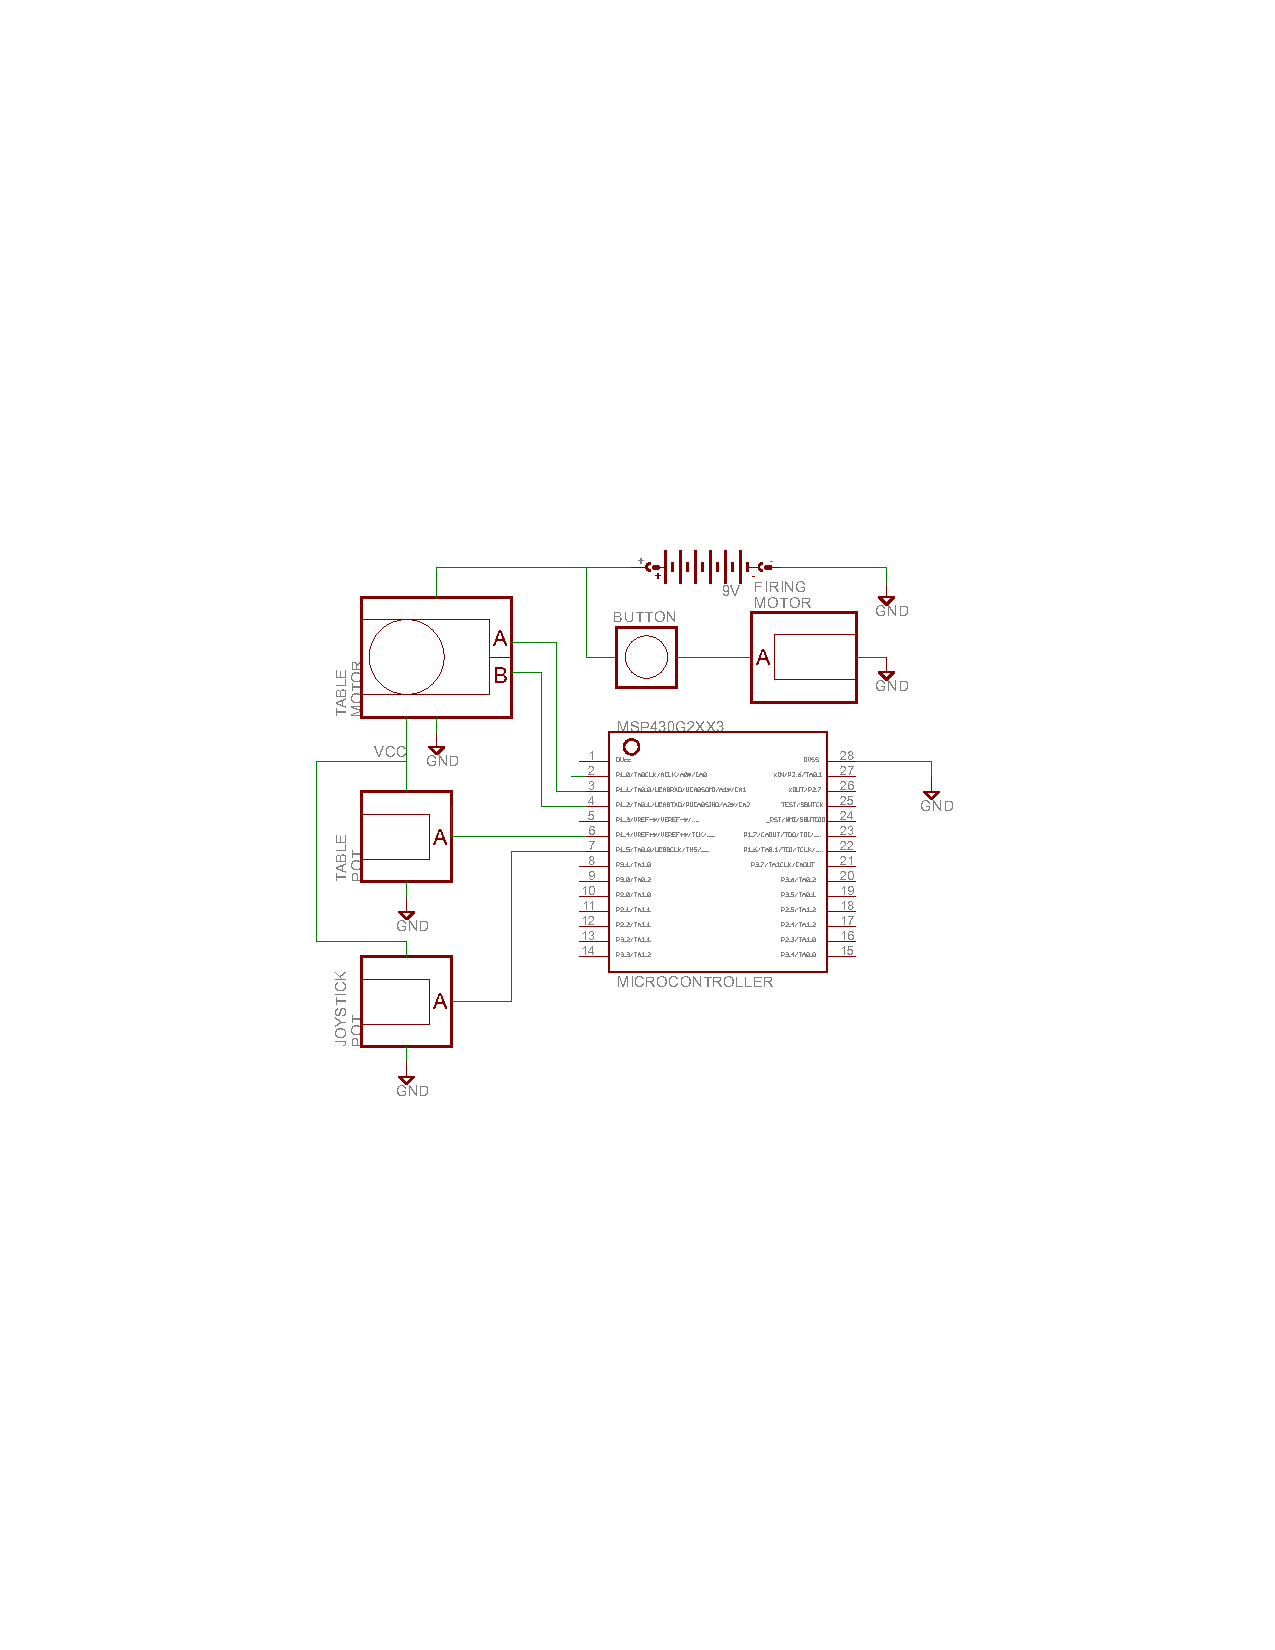
\includegraphics{report-images/high-level-diagram}
		\vspace{-9.5cm}
		\caption{High Level Diagram}
	\end{figure}

\newpage
	\subsection{Table Motor}
	\begin{figure}[!ht]
		\centering
		\vspace{-4cm}
		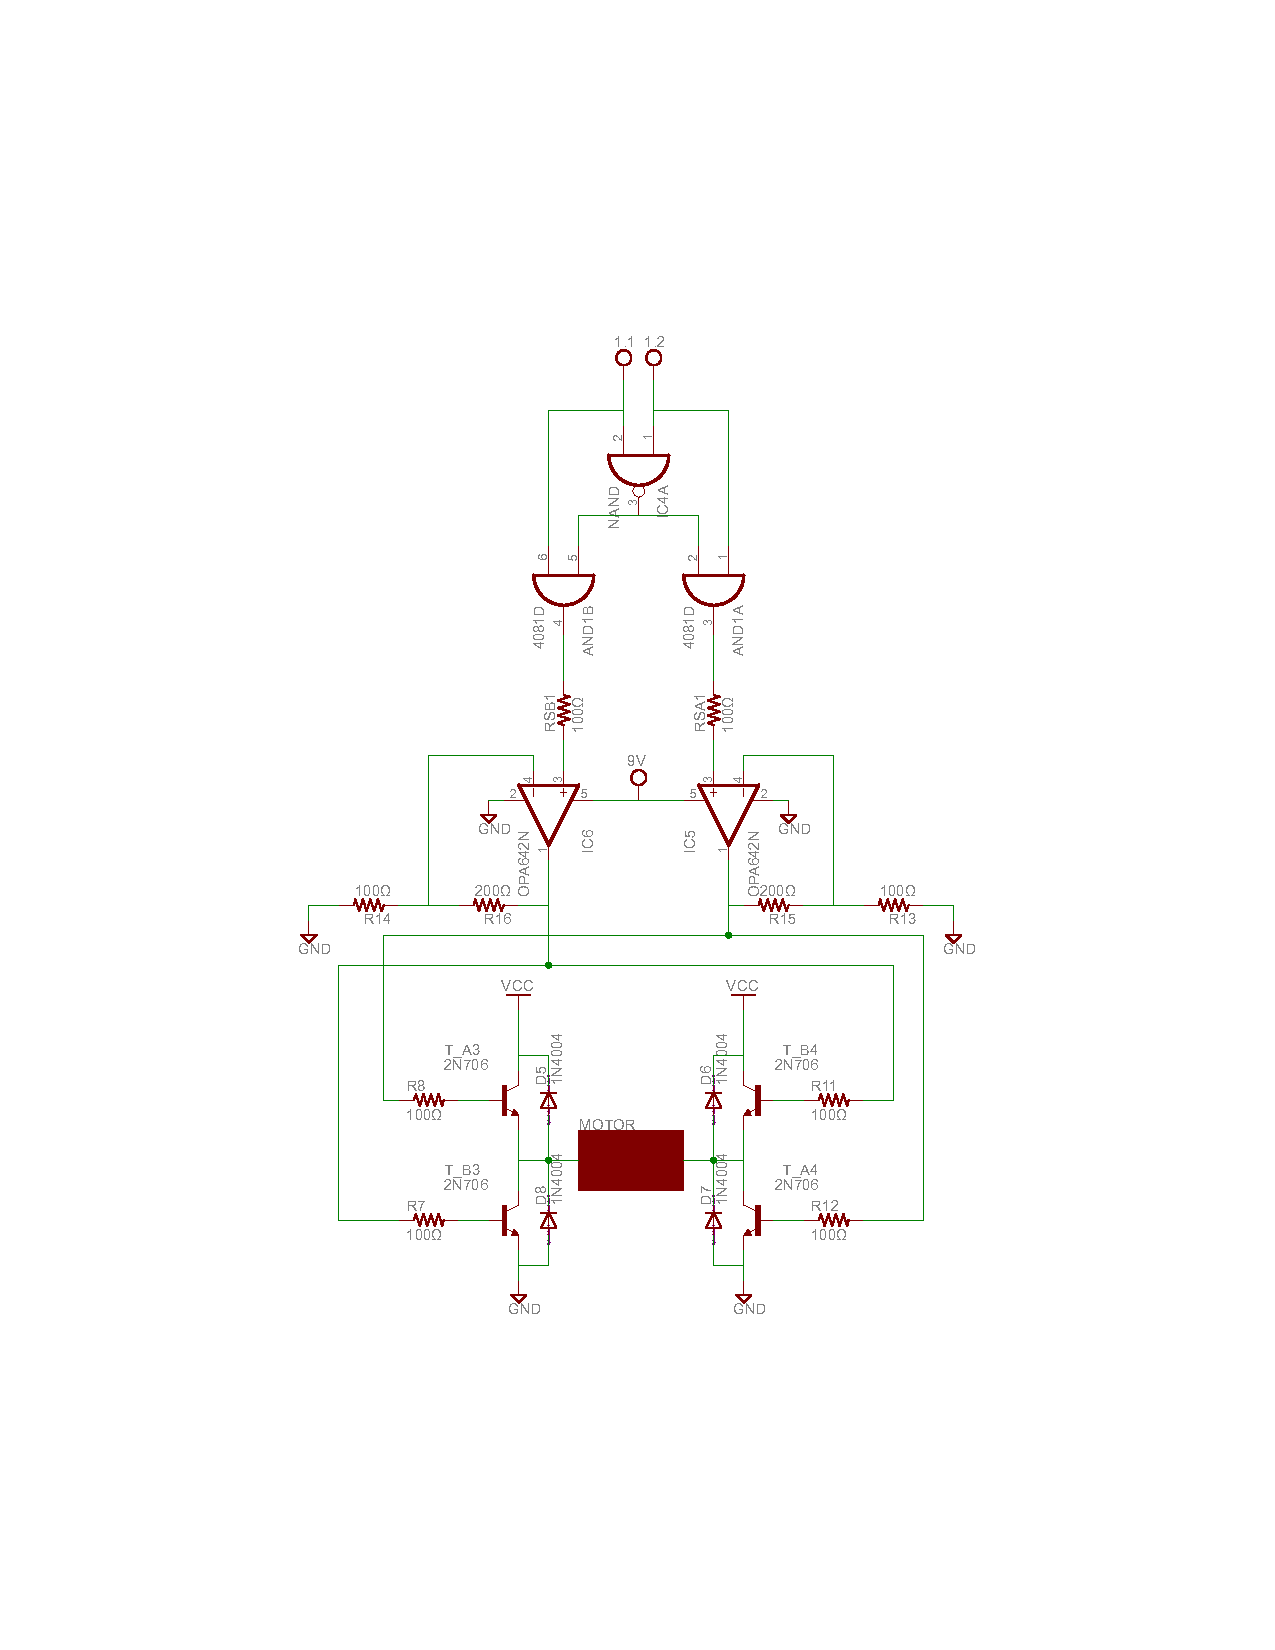
\includegraphics[scale=.8]{report-images/bidirectional-motor-driver}
		\vspace{-4cm}
		\caption{Table Motor Control}
	\end{figure}
	\noindent The motor control consists of an H-bridge (bottom half) for rotation in both directions.  The motor is protected from double-input by logic gates (top half).  The initial construction of the H-bridge did not provide sufficient power to drive the motor, so we used more transistors to make Darlington pairs (instead of restarting the bridge with PNP transistors).
\newpage
	\subsection{Potentiometers}
	\begin{figure}[!ht]
		\centering
		\vspace{-11cm}
		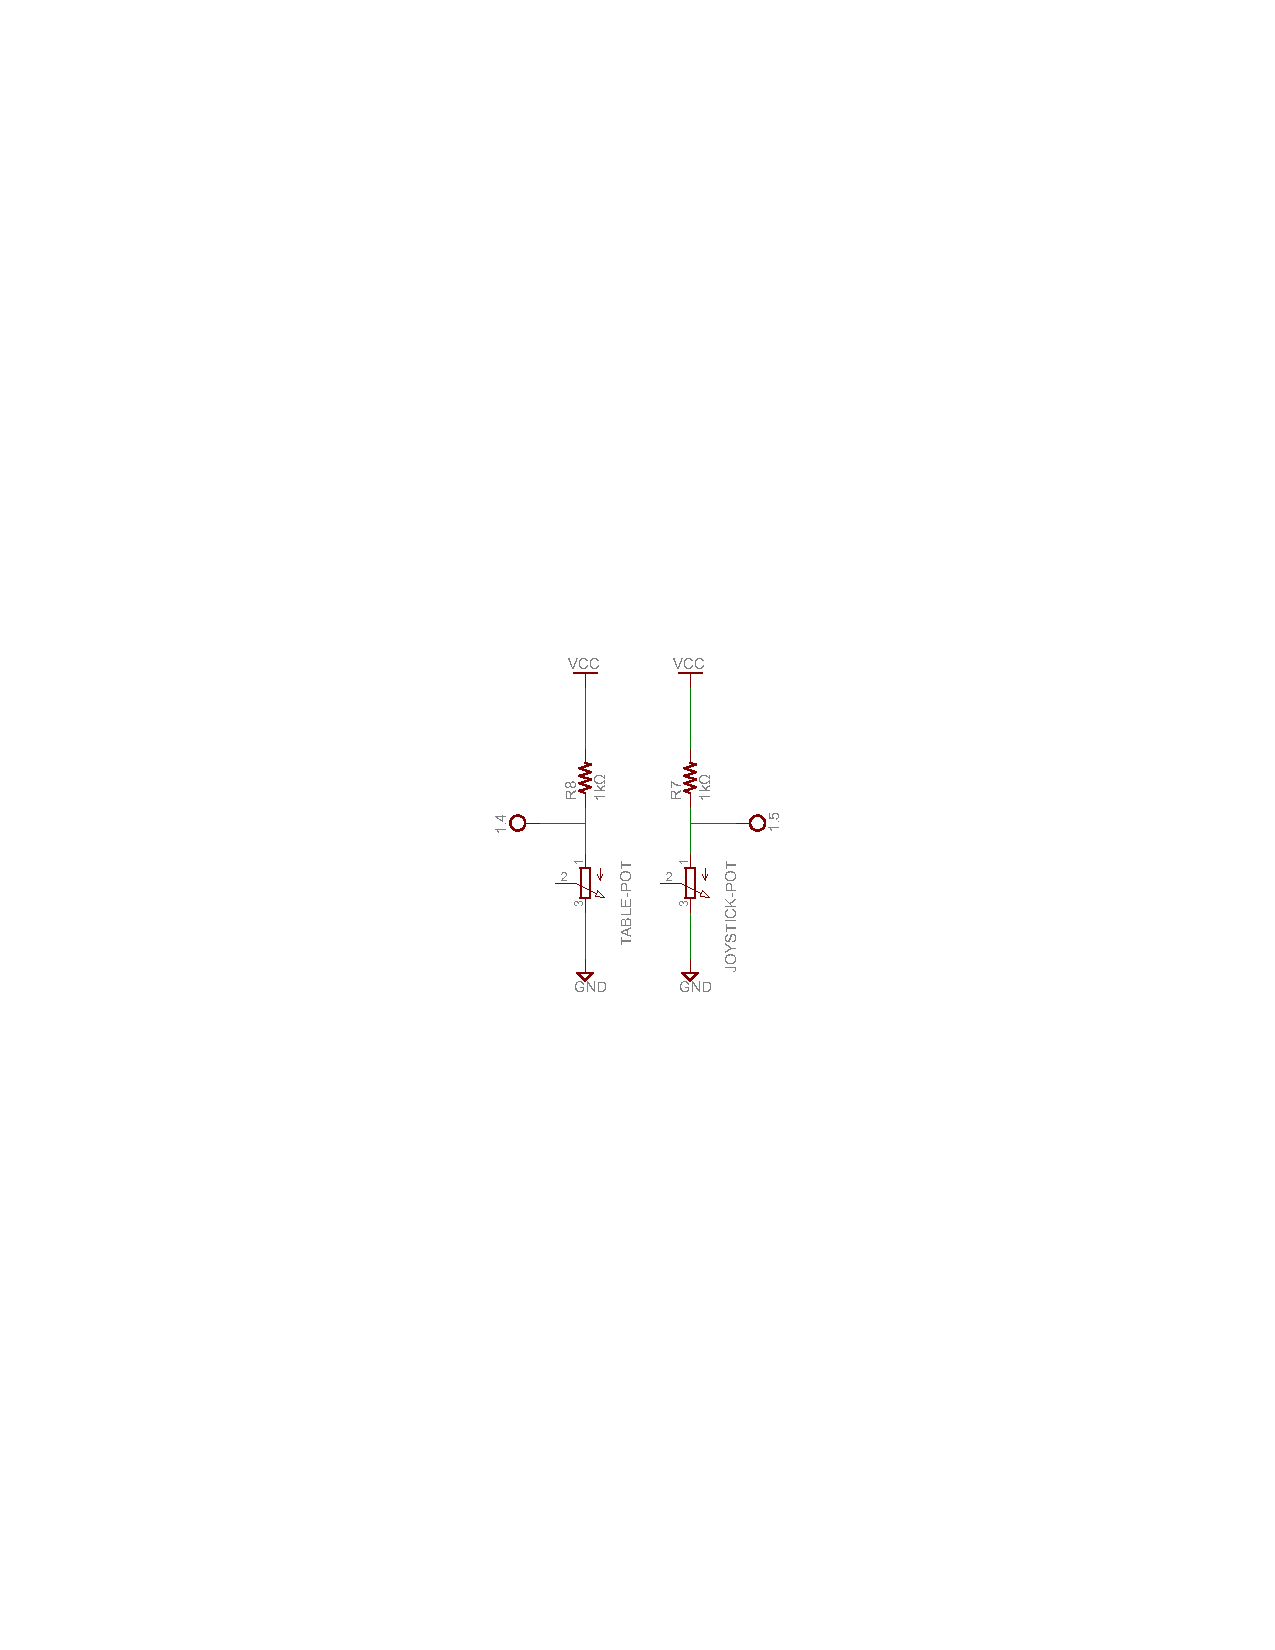
\includegraphics{report-images/potentiometers}
		\vspace{-11.25cm}
		\caption{Potentiometers}
	\end{figure}
	\noindent The MSP analogReads the voltage between the resistor and the potentiometer to determine the rotation of the potentiometer.  That in turn is used as input for control to match the two potentiometers.  
	\subsection{Firing Button}
	\begin{figure}[!ht]
		\centering
		\vspace{-10cm}
		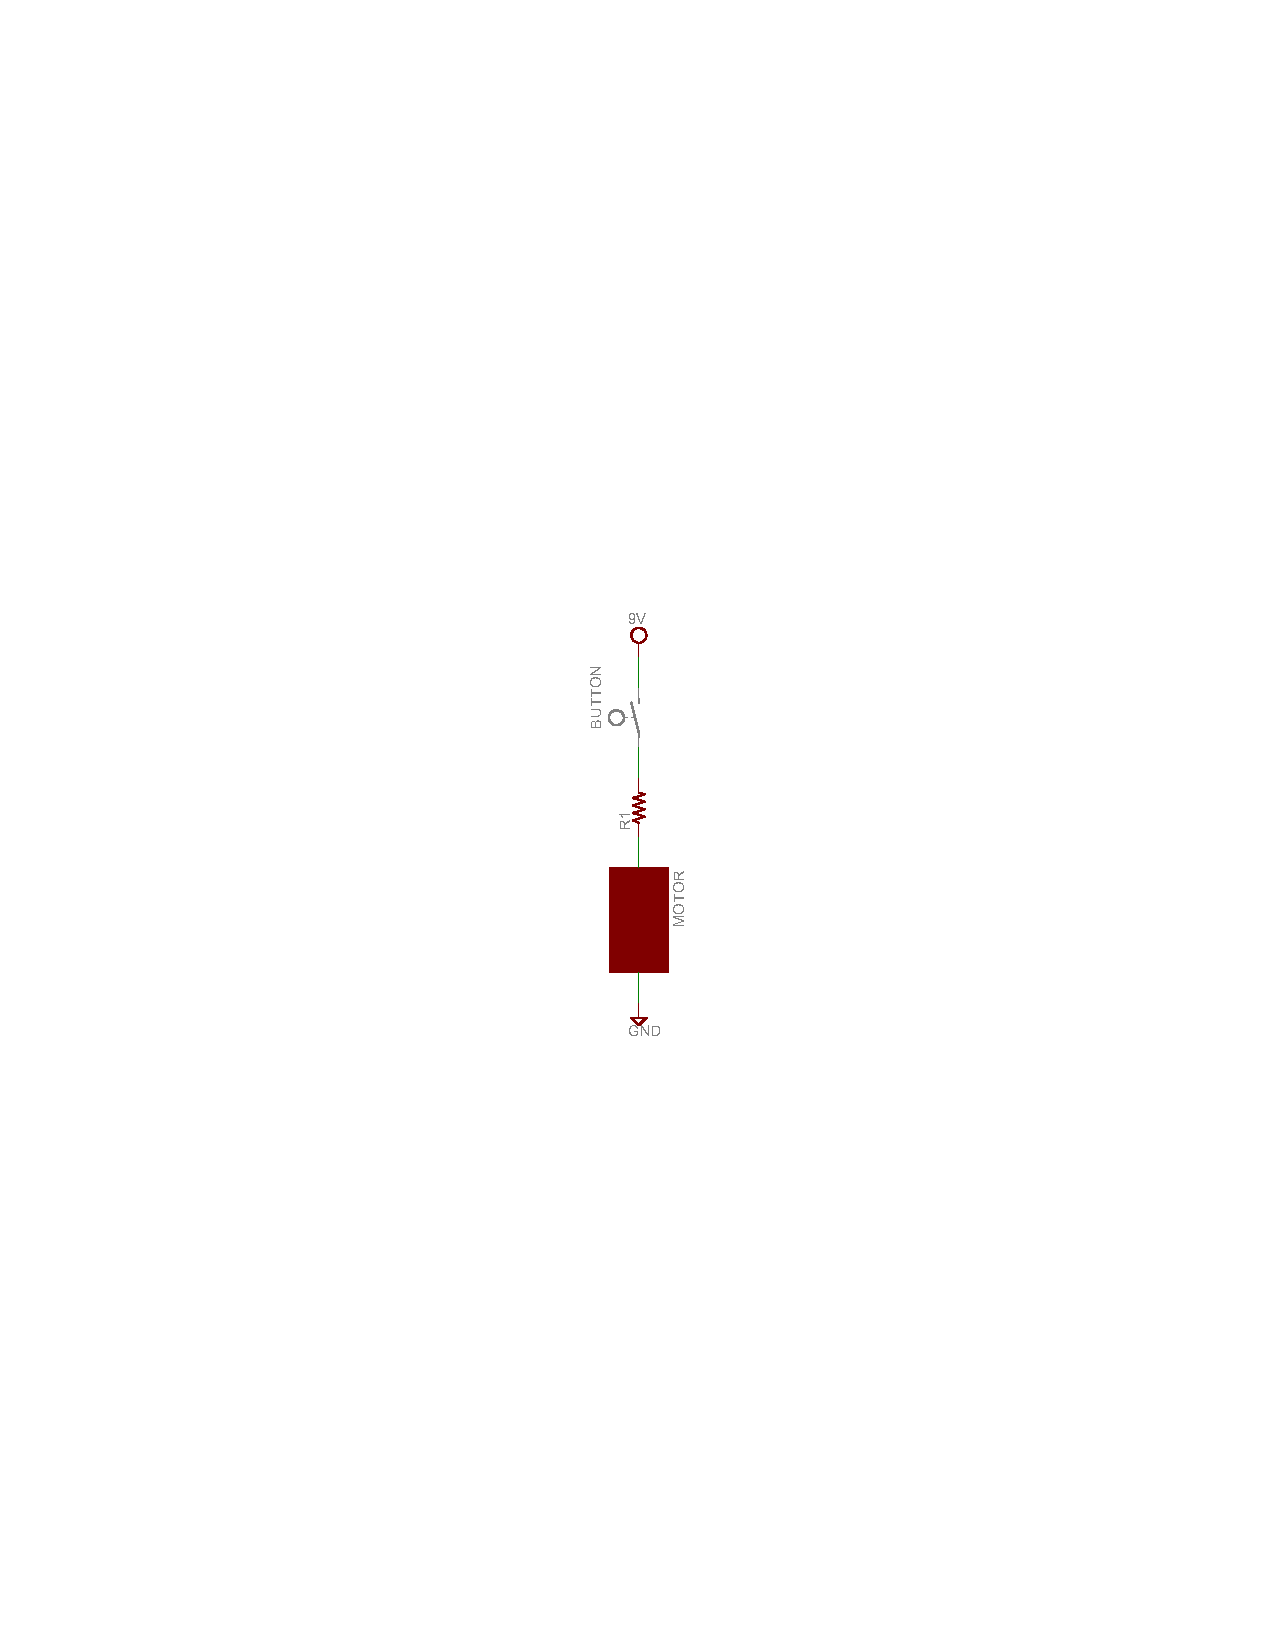
\includegraphics{report-images/firing-button}
		\vspace{-10.5cm}
		\caption{Firing Button}
	\end{figure}
	\noindent The button and its protection are directly linked to the motor.  The motor used for this obviated the need for a diode/transistor protection setup.
\newpage
\section{Code}
	\begin{lstlisting}
/**************/
/*** code.c ***/
/**************/
				
// Pins
int motor1a = P1_1; // Don't use 2_3 or 2_4
int motor1b = P1_2;
int potJoy = P1_5;
int potSensor = P1_4;
		
// Constants
int sensorTolerance = 0.1;
		
int main(){
	// LEDs used for testing/demo purposes
	pinMode(GREEN_LED, OUTPUT);
	pinMode(RED_LED, OUTPUT);
	
	pinMode(P1_1, OUTPUT);  // motor one way
	pinMode(P1_2, OUTPUT);  // motor other way
	pinMode(P1_5, INPUT);    // joystick potentiometer
	pinMode(P1_4, INPUT);    // table potentiometer
	
	int potJoyVal = 0;
	int potSensorVal = 0;
			
	while(1){
		// Reads the two potentiometer values
		potJoyVal = analogRead(potJoy);
		potSensorVal = analogRead(potSensor);
				
		// Handles differences in potentiometer readings to choose the
		// direction of rotation
		if(abs(potJoyVal - potSensorVal) < sensorTolerance){
			digitalWrite(motor1a, LOW);
			digitalWrite(motor1b, LOW);
			digitalWrite(RED_LED, LOW);
			digitalWrite(GREEN_LED, LOW);
		}
		else if (potJoyVal > potSensorVal){
			digitalWrite(motor1a, HIGH);
			digitalWrite(motor1b, LOW);
			digitalWrite(RED_LED, HIGH);
			digitalWrite(GREEN_LED, LOW);
		}
		else {
			digitalWrite(motor1a, LOW);
			digitalWrite(motor1b, HIGH);
			digitalWrite(RED_LED, LOW);
			digitalWrite(GREEN_LED, HIGH);
		}
		delay(100);
	}
}
	\end{lstlisting}
\end{document}